\section{Beyond Lossless Speculation: OS Hyperparameter Tuning Environment}
\label{sec:os-speculation}
Thus far, our experiments have focused on \emph{lossless} speculation, where speculative actions are validated sequentially before commitment. We now turn to a \emph{lossy} setting that relaxes this constraint.
In latency-sensitive environments like an operating system, 
waiting for a powerful but slow Actor (10-15s deliberation) can leave the system in a degraded state.
Instead, we use a fast Speculator to apply immediate provisional adjustments while the Actor deliberates. 
This is made safe by a last-write-wins mechanism—the Actor's final decision 
simply overwrites any speculative action, 
removing the need for complex rollbacks. 
This method accelerates convergence and improves reaction time, 
which we evaluate on the \texttt{sysbench cpu} benchmark, a CPU-bound workload~\citep{sysbench}.
%Our framework extends the work of~\cite{liargkovas2025llmTuning}, by introducing a fast, speculative loop to mitigate the deliberation latency of the expert Actor.
\subsection{Experimental Setup}
We tune Linux's Completely Fair Scheduler (CFS) parameter \texttt{min\_granularity}, 
which controls a task's minimum timeslice. 
This knob strongly affects scheduling performance: smaller timeslices reduce latency but can degrade throughput, yielding a classic trade-off. Building on~\citep{liargkovas2025llmTuning}, we augment the prior LLM-based tuning setup with a speculative control loop.
% Prior work~\citep{liargkovas2025llmTuning} demonstrated that an LLM-based agent can optimize this parameter; here, we extend that setup with a speculative control loop.
% Our system consists of a fast Speculator and a slow Actor. 

The Speculator proposes a parameter update each second using the latest performance metric. 
The Actor, in contrast, responds every 10–15 seconds after analyzing a compressed chronology of the Speculator's recent (measurement, action) pairs.
Upon arrival, the Actor’s decision is applied immediately and its state resets the Speculator’s context, preventing drift from the validated narrative.

\vspace{-5pt}
\paragraph{Evaluation}
%\vspace{-5pt}
We evaluate three systems: (1) \textbf{Actor-only}: slow but deliberative (10-15\,s interval); (2) \textbf{Speculator-only}: fast (1\,s interval) but non-extensive; (3) \textbf{Speculator–Actor}: combined system using speculative updates between Actor decisions.
% We are interested in (i) reaction time, (ii) convergence speed to the optimal setting, and (iii) ability to avoid local minima that trap the Speculator-only baseline.


\subsection{Results}
\begin{figure*}[t]
 \centering % Center the entire figure content
 % --- Left Column: The Plot ---
 \begin{minipage}[c]{0.64\linewidth}
  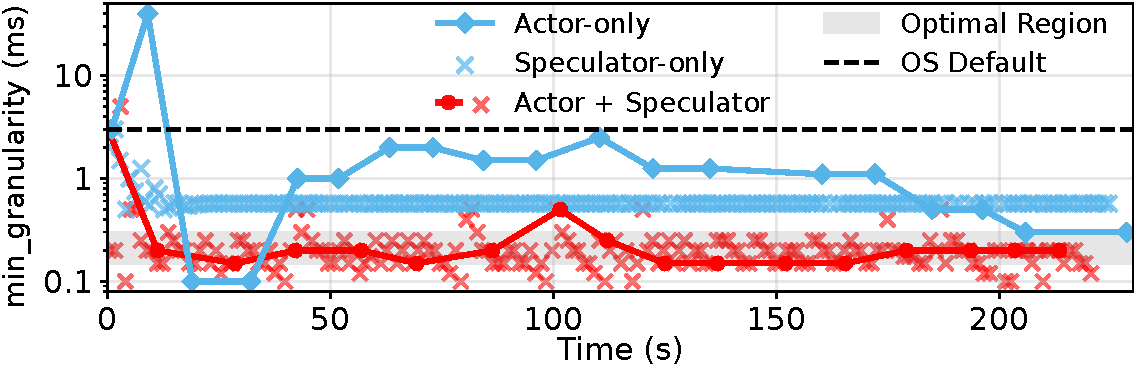
\includegraphics[width=\linewidth]{figures/os_tuning/combined_plot.pdf}
 \end{minipage}
 \hfill % Adds a flexible space between the two columns
 % --- Right Column: The Table ---
 \begin{minipage}[c]{0.35\linewidth}
  \centering
\begin{tabular}{l p{1.29cm}}
  \toprule
  \textbf{Configuration} & \textbf{Latency p95 (ms)} \\
  \midrule
  Untuned & 102.97\\
  Actor-only      &  54.00 \\
  Actor + Spec.   &  37.93 \\
  \bottomrule
\end{tabular}
 \end{minipage}
 \caption{
 \textbf{(Left)} Comparison of \textbf{Speculator-Actor}, \textbf{Speculator-only}, and \textbf{Actor-only} convergence.
 The Speculator shortens time spent exploring poor settings. 
 The Speculator-only agent stabilizes quickly but at a worse final value.
 \textbf{(Right)} Average p95 latency over a 20-second tuning experiment showing that rapid reaction offers immediate performance benefits (see \S\ref{app:speculative-mitigation}). Lower is better.}
 \label{fig:os-speculation}
 \vspace{-10pt}
\end{figure*}

% \paragraph{Speculator mitigates poor-reaction slowdowns} The Speculator dramatically improves reaction time, as observed Figure \ref{fig:os-speculation}~(Right). During the recovery period, the full Speculator-Actor system maintains an average p95 latency of 37.93 ms. This is a substantial improvement over the Actor-only baseline, which was forced to endure the poor performance for much longer and averaged 54.00 ms. The Speculator's rapid correction prevents the system from lingering in a high-latency state (initially 102.97 ms), providing immediate benefits while the slower Actor deliberates (the full experiment is detailed in \S\ref{app:speculative-mitigation}).
% \vspace{-5pt}
% \paragraph{Speculator accelerates convergence to optimum}
% The Speculator's high-frequency updates also significantly accelerate convergence. 
% As shown in Figure~\ref{fig:os-speculation} (Left), the Speculator-Actor system reaches an optimal setting (e.g., 0.2\,ms \texttt{min\_granularity}) in approximately 10–15 seconds. 
% In contrast, the Actor-only agent takes around 200 seconds---20x slower---and remains trapped in highly suboptimal states (e.g., latency $>$120\,ms) for a long period of time. 
% The Speculator's rapid exploration provides the Actor with a richer performance landscape, allowing it to steer the system away from these pathological regions more quickly.

% \vspace{-5pt}
% \paragraph{Speculator-only is good, but not optimal}
% Figure~\ref{fig:os-speculation} also shows that while the Speculator-only system reacts quickly, it converges prematurely to a suboptimal configuration: \texttt{min\_granularity} of 0.55\,ms (36.24\,ms latency). 
% This is significantly worse than the 0.2\,ms (30.26\,ms latency) achieved by the full Speculator-Actor system. Without the Actor's guidance, the Speculator lacks the reasoning depth to escape this local minimum.
% \vspace{-5pt}
% \paragraph{Cost and latency can both decrease.}
% Because the Speculator acts as a fast explorer that accelerates convergence, the \emph{total} cost can in fact be \emph{lower}, despite launching additional speculative branches. 
% % By reaching a correct trajectory much earlier, the system avoids the prolonged high-latency exploration incurred by the Actor-only baseline.
% As shown in Table~\ref{tab:os}, the Actor-only baseline converges at roughly $200\text{s}$ with a total cost of $2.18$ cents, whereas the Actor+Speculator method converges around $13\text{s}$ with a total cost of only $0.17$ cents.

% The joint Speculator–Actor system combines fast adaptation with strategic guidance, achieving both responsiveness and optimal steady-state performance.


% \vspace{-5pt}
\paragraph{Speculator mitigates poor-reaction slowdowns.}
As shown in Figure~\ref{fig:os-speculation} (right), the Speculator significantly improves reaction time. 
During recovery, the full Speculator–Actor system maintains an average p95 latency of 37.93\,ms, compared to 54.00\,ms for Actor-only, which remains longer in degraded states (initially 102.97\,ms). 
Fast speculative updates provide immediate mitigation while the Actor deliberates (details in \S\ref{app:speculative-mitigation}).

\vspace{-5pt}
\paragraph{Speculator accelerates convergence to optimum.}
Figure~\ref{fig:os-speculation} (left) shows that the joint system reaches the optimal setting (0.2\,ms \texttt{min\_granularity}) in 10-15\,s, whereas Actor-only requires $\sim$200\,s and remains trapped in highly suboptimal regions (e.g., latency $>120$ms) for extended periods. 
Rapid speculative exploration helps the Actor avoid pathological configurations.

\paragraph{Speculator-only reacts quickly but is suboptimal.}
While Speculator-only stabilizes rapidly, it converges to a worse configuration (0.55\,ms; 36.24\,ms latency) than the joint system (0.2\,ms; 30.26\,ms). 
Without the Actor’s deeper reasoning, it cannot escape local minima.

\paragraph{Cost and latency both decrease.}
Despite additional speculative calls, total cost is lower due to faster convergence. 
As shown in Table~\ref{tab:os}, Actor-only converges at $\sim$200\,s with a total cost of 2.18\,cents, whereas Speculator–Actor converges in $\sim$13\,s with only 0.17\,cents.

Overall, the joint system combines fast adaptation with strategic guidance, achieving both responsiveness and optimal steady-state performance.